\section{Model Exercise 2-1b (02): Fluid driven percolation in clay}
\label{sec:mex2-1b}
%------------------------------------------------------------------------------
\Authors{Amir Sattari, Keita Yoshioka et al.}
%------------------------------------------------------------------------------
As describe in the section \ref{The Fluid Driven Percolation in Claystone from Mont-Terri (CAU Kiel)}, the fracking path and pressure are determined for the cubic sandy Opalinus claystone samples under various stress configuration. In addition to the stress configuration and due to the high anisotropy of the claystone, in here, the effect of the embedded layering orientation on the fracking paths is also investigated. It is expected that due to the weak bond between the layers, the fracking path and flow channels be in the embedded layering surfaces. 
%------------------------------------------------------------------------------
\subsection{Experimental set-up}
%------------------------------------------------------------------------------
The cubic Opalinus claystone samples are prepared in the side dimension of 43 $mm$ and with the drilled cavity length and diameter of 20 and 8 $mm$. The mechanical stress configurations are as shown in \ref{fig:Amir_Percolation_Stress_1} and \ref{fig:Amir_Percolation_Stress_2}. The syringe pump is used to pump the pressurized hydraulic oil (up to 517 $Bar$) into the sample and with gradually increasing the pressure the fracking test is carried out. In the first setup, the hydraulic fracking is initiated at 23 $MPa$ and the clear flow paths through the embedded layering surfaces is seen \ref{fig:Amir_Percolation_Frack1a} and \ref{fig:Amir_Percolation_Frack1b}. 

\todo[inline]{[CAU]: Please add / refer to experimental results}
%------------------------------------------------------------------------------
\subsection{Model approaches}
%------------------------------------------------------------------------------
\subsubsection*{Lattice-Element-Model (LEM)}

With the LEM, the effect of the claystones anisotropy on the fracking paths and fracking pressure is investigated. The similar approach as described in section \ref {sec:mex01} is taken to define the layering orientations in the medium. It is assumed that the interface elements bonding two different layers have 5 times weaker strength than the same layers bond. The generated 3D setup using the LEM is shown in Figure???. The percolation tests under a same stress configuration, \ref{fig:Amir_Percolation_Stress_1} , but with the two different embedded layering orientations are simulated. The Figure??? and Figure??? show the fracking path and flow rate under the 1st stress configuration, when the embedded layers are perpendicular to the injection direction. Similarly, Figure??? and Figure??? depict the fracking path and flow rate when the embedded layers are parallel to the injection direction.

\todo[inline]{[CAU]: Please add LEM simulation results}

\subsubsection*{Finite-Element-Model: Variational Phase-Field (VPF)}

A computational domain for the variational phase-field model is depicted in Fig~\ref{fig:VPF_init}.
Relying on the symmetry of the domain, 1/4 of the domain was simulated. 
The whole domain was discretized with first-order tetrahedral elements.
The total element count is 27,917,126 with 5,432,325 nodes.
Two scenarios of boundary loading were simulated and simulated crack developments are shown in Figs~\ref{fig:Keita_ME2_VPF_case1} and~\ref{fig:Keita_ME2_VPF_case2} and the corresponding pressure responses are in Fig~\ref{fig:Keita_ME2_VPF_pres}.

\begin{figure}[!ht]
\centering
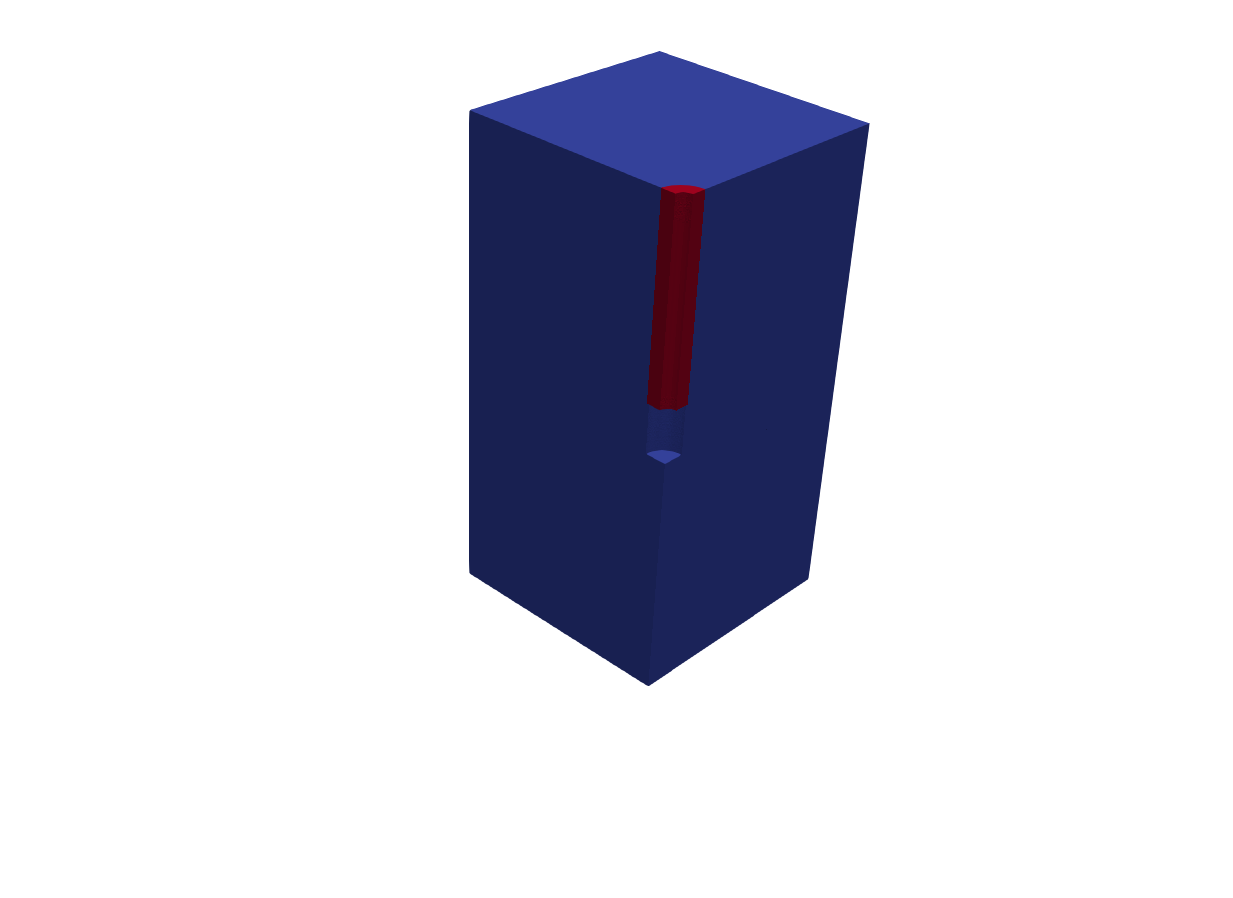
\includegraphics[width=1.0\textwidth]{figures/VPF_init.png}
\caption{A computational domain for the variational phase-field model.}
\label{fig:VPF_init}
\end{figure}

\begin{figure}[!ht]
\begin{subfigure}[c]{0.48\textwidth}
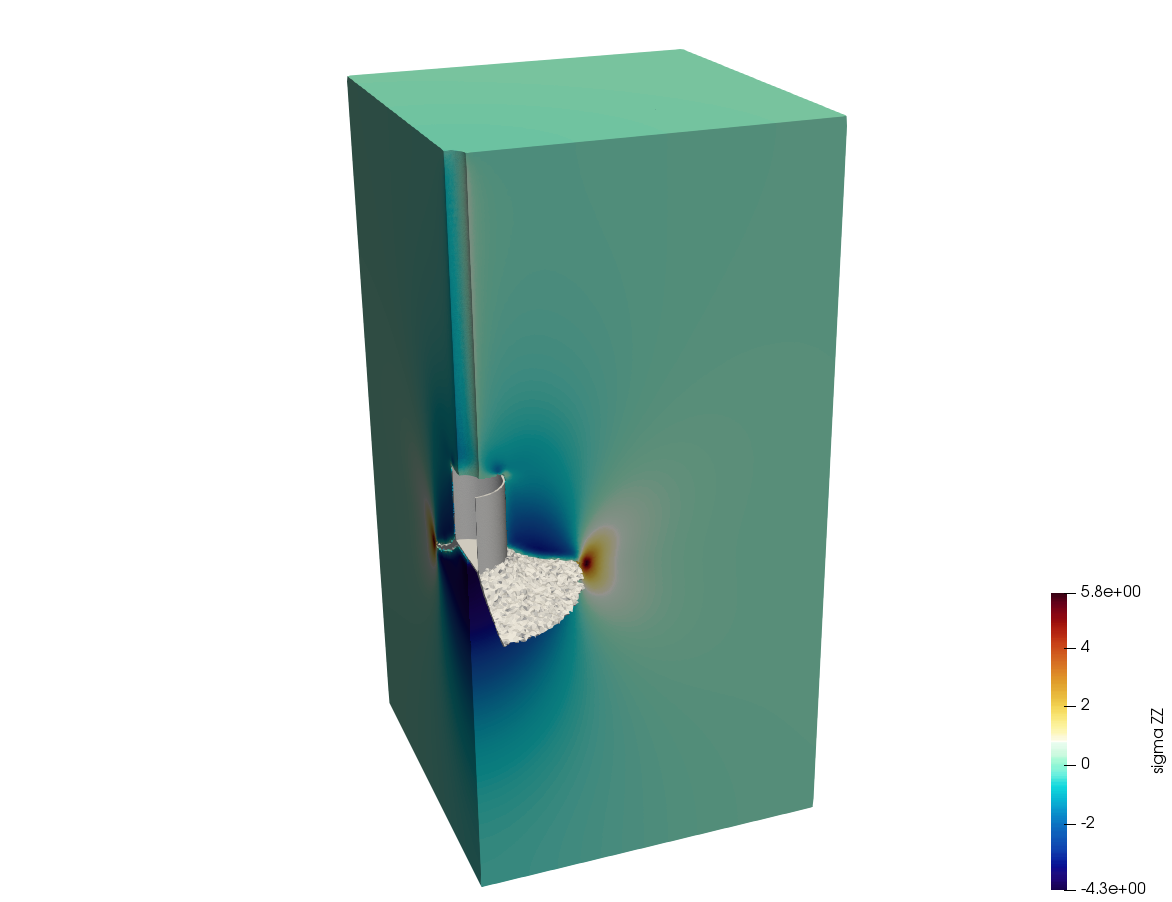
\includegraphics[width=1\textwidth]{figures/Keita_ME2_case1.png}
\subcaption{}
\label{fig:Keita_ME2_VPF_case1_zoomout}
\end{subfigure}
\hfill
\begin{subfigure}[c]{0.48\textwidth}
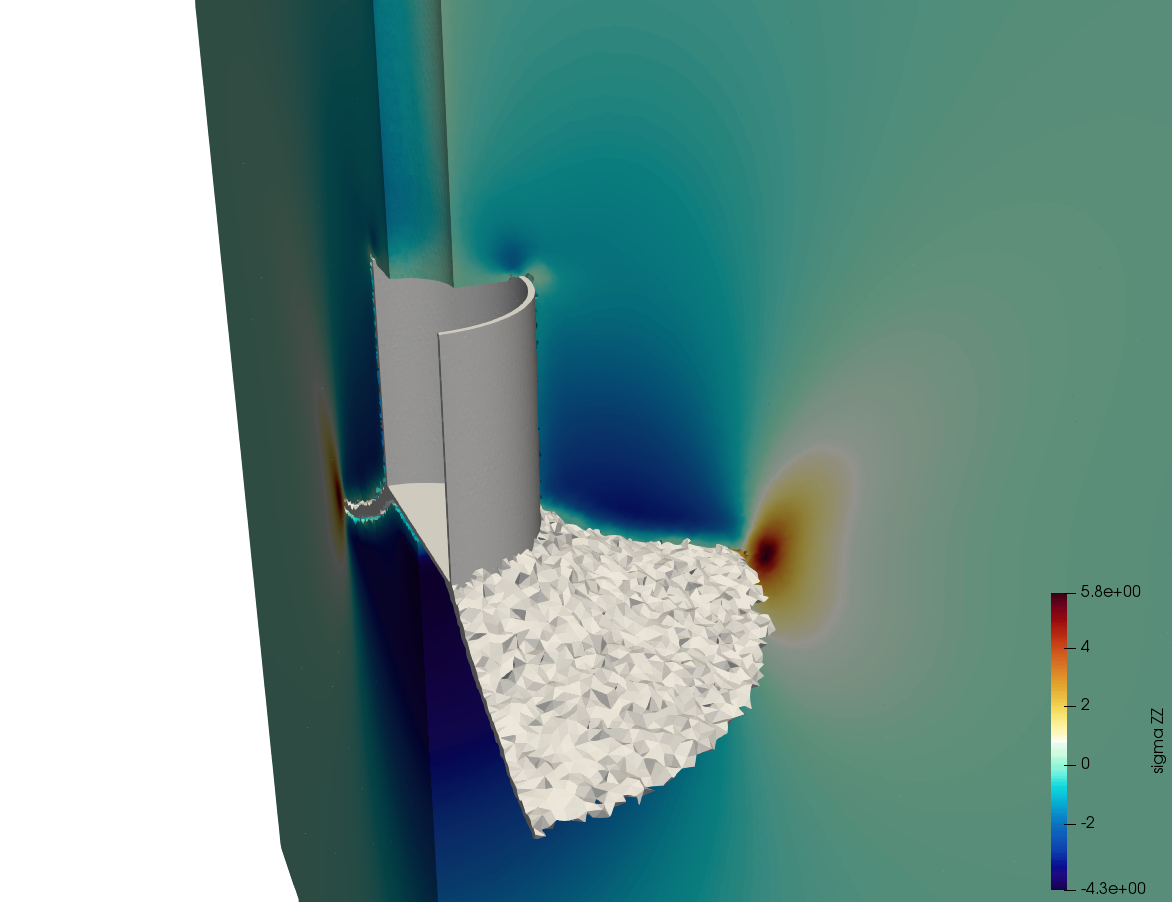
\includegraphics[width=1\textwidth]{figures/Keita_ME2_case1_zoomin.png}
\subcaption{}
\label{fig:Keita_ME2_VPF_case1_zeemin}
\end{subfigure}
\caption{The simulation of fluid driven percolation for case1. Created fracture and the vertical stress are shown.}
\label{fig:Keita_ME2_VPF_case1}
\end{figure}

\begin{figure}[!ht]
\begin{subfigure}[c]{0.48\textwidth}
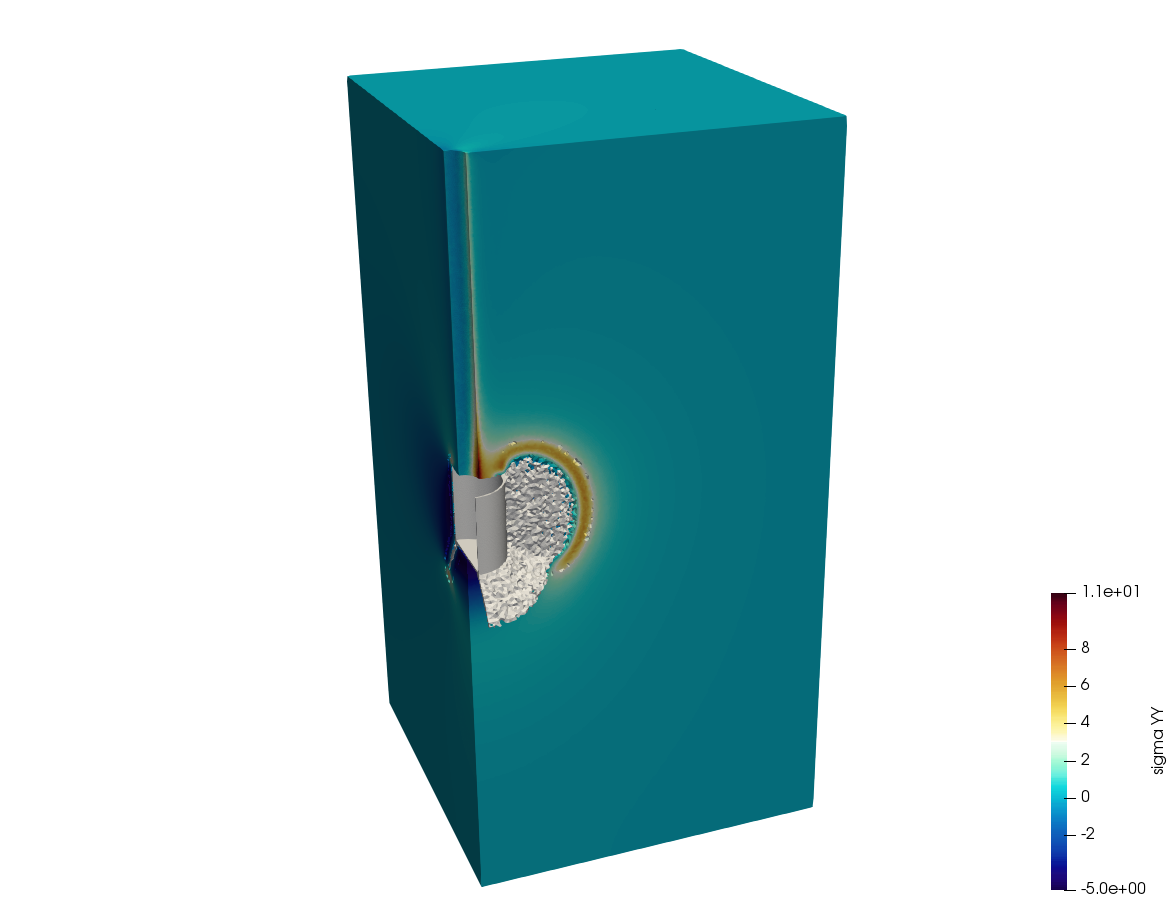
\includegraphics[width=1\textwidth]{figures/Keita_ME2_case2.png}
\subcaption{}
\label{fig:Keita_ME2_VPF_case2_zoomout}
\end{subfigure}
\hfill
\begin{subfigure}[c]{0.48\textwidth}
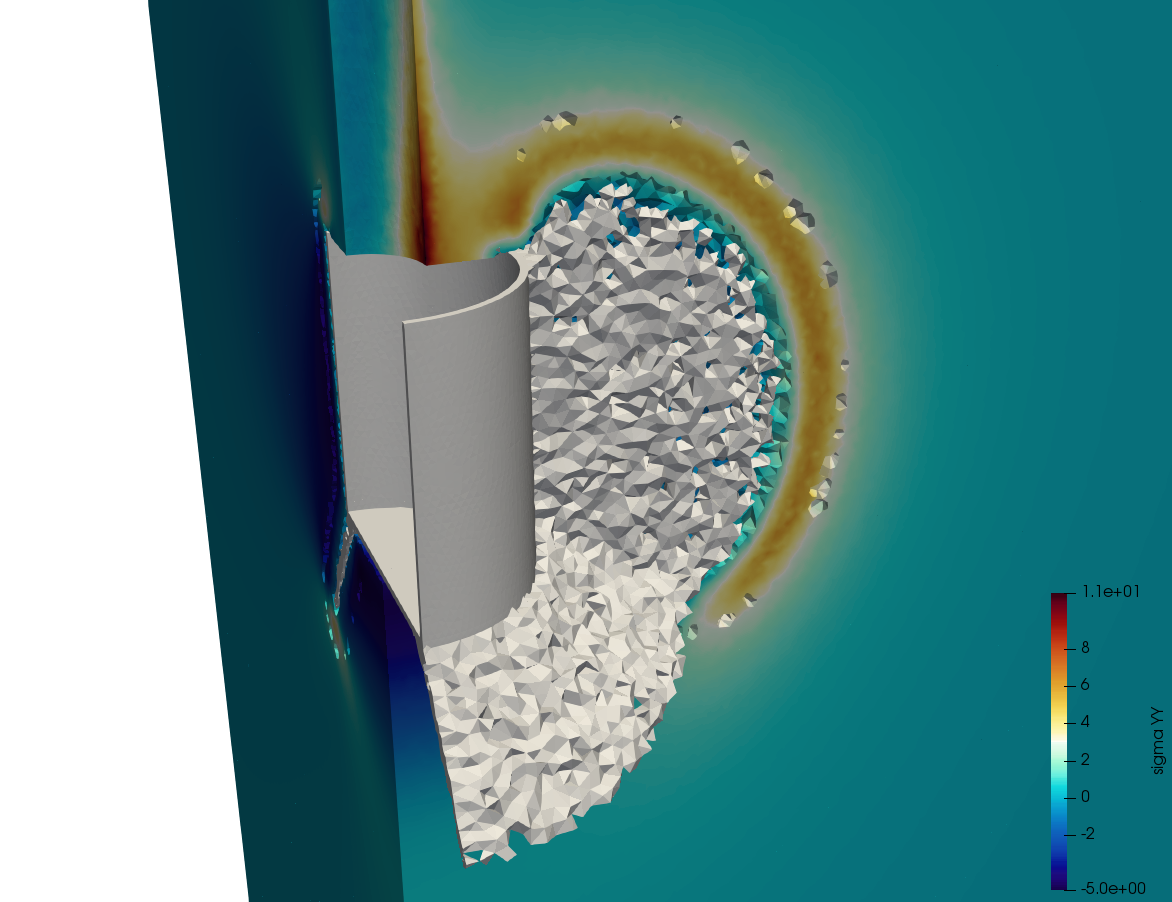
\includegraphics[width=1\textwidth]{figures/Keita_ME2_case2_zoomin.png}
\subcaption{}
\label{fig:Keita_ME2_VPF_case2_zeemin}
\end{subfigure}
\caption{The simulation of fluid driven percolation for case2. Created fracture and the horizontal stress are shown.}
\label{fig:Keita_ME2_VPF_case2}
\end{figure}

\begin{figure}[!ht]
\centering
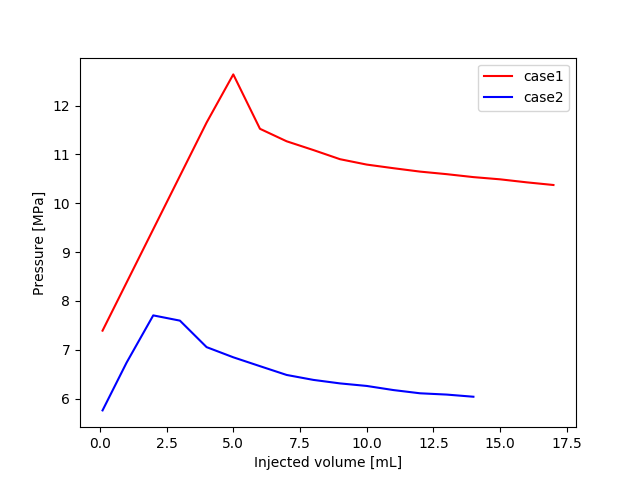
\includegraphics[width=1.0\textwidth]{figures/Keita_ME2_pressures.png}
\caption{Pressure responses from the variational phase-field simulations.}
\label{fig:Keita_ME2_VPF_pres}
\end{figure}

%------------------------------------------------------------------------------
\subsection{Results and discussion}
%------------------------------------------------------------------------------
